\chapter{Business Context}\label{chapter:business}

\section{Limit Order Book}
% Definition
This section explains the definition of the limit order book, its price mechanism and market impact, key challenges such as cancellations and hidden orders, and stylized facts, including volatility clustering, long memory in order flow, and the convergence of prices. The limit order book is dynamic updates of transactions in \textit{order-driven marketplaces}, marking an evolution from \textit{quote-driven marketplaces}.

\subsection{Structure, Price Levels and Key Metrics}
The three pillars of limit order book data are time, price and volume. An order $x$ submitted at time $t$ represents a commitment to buy/sell up to a maximum volume $v$ with price $p$. Orders arrive in the set of queues \citep{gould_limit_2013}, where each remains active as either a buy or sell order until it is executed or canceled. 

% bid/ask direction, best bid/ask, 5 levels
The direction of price is an important aspect of the order book flow. The \textit{bid price} represents the price at which traders are willing to buy a given asset, while the \textit{ask price} represents the price at which traders are willing to sell. I only consider the first five price levels in this thesis, belonging to bid/ask price respectively. They are denoted as $\{P_B ^ {i}$, $i = 1, \dots, 5\}$ on the bid side, and $\{P_A ^ {i}$, $i = 1, \dots, 5\}$ on the ask side. From an order book perspective, the first level of bid price $P_B^1$ is the best (highest) bid where traders are willing to buy, while the first level of ask price $P_A^1$ is the best (lowest) ask where traders are willing to sell. As the level increases, bid prices decrease, and ask prices increase, indicating that traders are willing to buy at lower prices or sell at higher prices. The structure of limit order book at time $t$ is shown in the Figure~\ref{fig: order_book_t}. More elements in it will be illustrated below.

\begin{figure}[h]
    \centering
    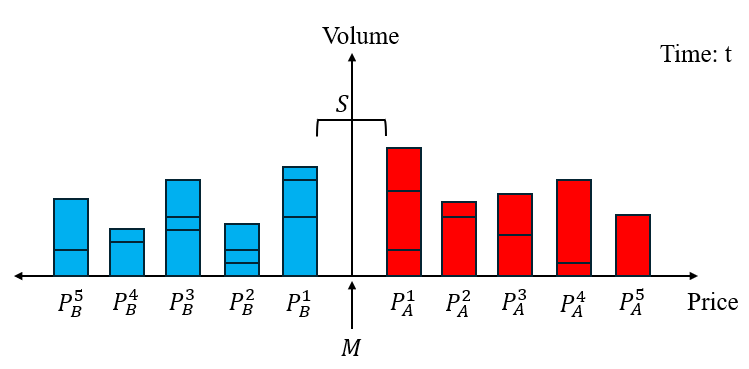
\includegraphics[width=0.8\linewidth]{figures/order_book_t.png}
    \caption{Limit Order Book Flow at Time t}
    \label{fig: order_book_t}
\end{figure}

From the perspective of buyers, placing orders in the bid range reflects a more neutral or passive opinion, as these orders wait to be matched rather than executed immediately. This provides liquidity to the market. Conversely, when buyers want to execute orders more aggressively, they place orders at the ask price range, increasing the likelihood of immediate execution. Aggressive buy orders take ask orders out of the order book flow and consume market liquidity. In other words, $P_A ^ {1}$ is the lowest price at which it is immediately possible to buy the traded asset. This also leads to a concept of \textit{market orders}, contrary to which are the \textit{limit orders}. Market orders stand for orders which are filled immediately after submission, while limit orders become the available liquidity active in the order book. However, aside from immediacy of execution, there is no fundamental difference between the two order types. The same mechanism applies to sellers, where passive sell orders provide liquidity at the ask price, while aggressive sell orders execute against bid prices.

The \textit{bid-ask spread} $S$ and \textit{mid-price} $M$ are fundamental metrics derived from the best bid price $P_B ^ {1}$ and best ask price $P_A ^ {1}$. Despite their mathematical simplicity, as expressed in Equations \ref{eq:spread} and \ref{eq:mid price}, these two metrics play a crucial role in the \gls{microstructure of financial markets}, much like how the Einstein field equations support the theoretical framework of general relativity. They serve as a bridge between market activity interface and the underlying mechanisms of price formation, liquidity, and trading dynamics. Every study on the limit order book certainly involves these measures, as they illustrate essential market characteristics.
\begin{align}
    S = P_A ^ {1} - P_B ^ {1}  \label{eq:spread}\\
    M = (P_A ^ {1} + P_B ^ {1})/2
    \label{eq:mid price}
\end{align}

The bid-ask spread is a key indicator of market liquidity and transaction costs. A narrower spread suggests higher liquidity and lower execution costs, while a wider spread may indicate market inefficiencies or heightened uncertainty \citep{GLOSTEN198571}. Moreover, changes in the spread are closely linked to market sentiment, as it tends to widen during periods of volatility and tighten when market conditions stabilize.

The mid-price, on the other hand, is a fair valuation across the order book flow. It serves as a benchmark for price movements and is widely used in empirical research to model order flow dynamics, volatility, and high-frequency trading strategies. Statistical properties, like stability and convergence, of mid-price provide insights into price simulation and prediction. More stylized facts are demonstrated in Chapter~\ref{cp: facts}. 

\subsection{Price Mechanism and Market Impact}
%how to match, how to fill, how to disappear, auction
In the limit order book, price matching mechanism take the lead of the evolution of bid/ask prices over time. The most common rule is that orders follow a \textit{price-time priority}, meaning higher bid prices and lower ask prices get matched first. When multiple orders are placed at the same price, they are executed following a first-come, first-served rule. 

When a limit order is placed, it is not immediately matched and stays in the order book, adding liquidity and waiting for future trades. When a market order is placed, it is executed at the best available price on the opposite side of the book. If the order is larger than the available volume at that price, the rest moves to the next best level until it is fully executed, or no more matches are found. 

To illustrate the order book flow more clearly, Figure~\ref{fig: order_book_t_1} shows the state of the book at time $t+1$, following Figure~\ref{fig: order_book_t}. When a buy limit order is placed at bid price level 1 ($P_B^1$), it means a trader wants to buy but prefers a better price over immediate execution. This order follows the time priority and remains active until either the market moves downwards or aggressive traders occur to take this order out directly. But the order can only be filled after all earlier orders at the same price level are filled or canceled. Such a passive limit order does not cause $\{P_B ^ {i}$, $i = 1, \dots, 5\}$ or $\{P_A ^ {i}$, $i = 1, \dots, 5\}$ to change. 

\begin{figure}[h]
    \centering
    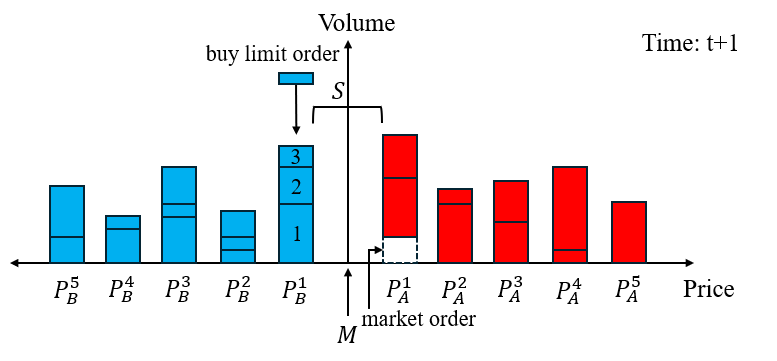
\includegraphics[width=0.8\linewidth]{figures/order_book_t_1.png}
    \caption{Limit Order Book Flow at Time t+1}
    \label{fig: order_book_t_1}
\end{figure}

There is also a market order filled at ask price level 1 ($P_A^1$) in Figure~\ref{fig: order_book_t_1}. This represents a trader who wants to buy aggressively, matching against the highest priority active sell order in the order book. As a result, it is executed immediately at $P_A^1$. Whether the best ask price ($P_A^1$) changes depends on how big the market order is compared to the number of active sell orders at $P_A^1$. If the market order is larger than the available sell volume at this price, the remaining part of the order will continue to match with the next best ask price ($P_A^2$), and then $P_A^3$, and so on. The process will continue until the entire order is filled. But in the case that there is a no-worse-than price applied to the market order, the process will end when there are no more sell orders at reasonable prices. If all the sell orders at $P_A^1$ are used up, the best ask price will move to the next available sell order ($P_A^2$) in the book. This means that large market orders can push prices up by removing sell orders at multiple levels.

Moreover, when a buy (respectively, sell) order is placed between best bid (respectively, ask) price and best ask (respectively, bid)price, it will cause the $\{P_B ^ {i}\}$ to move right and best bid price to increase (respectively, the $\{P_A ^ {i}\}$ to move left and best ask price to decrease). 

Other actions, such as canceling, changing, or placing new orders, along with order filling, constantly update the order book, influencing price movements and order book dynamics.

\subsection{Stylized Facts} \label{cp: facts}
%heavy-tailed, volatility clustering, long memory in order flow, autocorrelation, Brownian motion of mid-price
As mentioned at the end of Chapter 1.1.1, the limit order book exhibits various statistical properties which are the so-called \textit{stylized facts}. \cite{vyetrenko_get_2019} reviewed a wide range of stylized facts, but I focus on a concise subset that is the most relevant to limit order book simulation:
\begin{enumerate}
    \item Arrival rates: Orders do not arrive randomly but follow patterns. The frequency of order arrivals follows statistical patterns and is commonly modeled using point processes.
    \item Autocorrelation of price changes: Price changes tend to slightly reverse in the short term due to bid-ask spread effects, but over longer periods, price changes are mostly independent.
    \item Volatility clustering: When prices move a lot in one period, they tend to keep moving a lot in the next. When price changes are small, they stay small for a while.
    \item Heavy-tailed distributions: The distribution of price returns, order sizes, and waiting times exhibits heavy tails. Extreme values price movements happen more often than expected in a normal distribution.
    \item Average shape of the book: The number of buy and sell orders at different price levels is not balanced. Some price levels have more orders than others, creating a typical shape.
    \item Price paths: Prices do not move randomly but follow patterns influenced by order flow. Over long periods, mid-price is convergent to a Brownian motion in a complete limit order book. 
    \item Long memory in order flow: Buy and sell orders are not placed randomly. The way orders are placed, canceled, and executed depends on past order activity and follows long-term patterns.
\end{enumerate}


\subsection{Challenges in Limit Order Book}
Due to the high frequency of trading, the presence of algorithmic strategies, and the participation of multiple traders, studying \gls{lob} is difficult. There are various problems challenging the analysis. \cite{drame2020limitorderbooklob} thinks the presence of both informed and uninformed traders causes information asymmetry on \gls{lob} dynamics. \cite{gould_limit_2013} further discuss the balance between perfect rationality and zero intelligence when describing trader behavior. However, this section focuses on the structural and operational challenges of the \gls{lob} itself, particularly those that affect simulation and its application in back testing trading strategies.
\begin{enumerate}
    \item State-space complexity: The \gls{lob} has a huge number of possible states at any given moment. The continuous updates of orders results in a dynamic system with high-dimensional complexity, which increases the computationally difficult. To make analysis feasible, simplifying assumptions are necessary. But preserving essential structures and statistical properties of the \gls{lob} is also indispensable.

    \item Incomplete order book along with aggressive trades: The visible limit order book does not show all trading intentions. Additional transaction details exist in trade book data, which are not reflected in the standard order book view. On the one hand, it's because some \gls{venues} allow traders to submit hidden-size orders that do not appear in order book updates. But these hidden passive orders are not important in our backtesting. On the other hand, aggressive trading events shot specific orders immediately. Such orders tend to be market orders, directly taking active orders out. As a result, researcher can't make sure that the observed \gls{lob} are actually the real activities happening in the realistic market. To address this issue, trade book data can be compared with order book records to identify missing events, and efforts can be made to reconstruct the true order flow by incorporating aggressive trades.

    \item Cancellation: Studies have indicated that most orders end in cancellation rather than filling. This seems to show a high level of trader disappointment. However, cancellations are not always due to unfulfilled intentions, some traders place and then cancel orders on purpose in order to gauge market trends and hidden liquidity. The meaning of volume changes in the \gls{lob} vary: some orders are fully or partially filled, some are canceled, and others remain unchanged. These possibilities contribute to the complex volume dynamics at each price, making it difficult to distinguish order filling from cancellation. Trade book data is crucial in addressing this issue, as it provides additional information on whether volume changes result from actual trades or cancellations.

    \item Differences among venues: The \gls{lob} updates are different across venues due to variations in market structure and transparency. Some venues allow more hidden orders and do not provide detailed order messages, making it harder to reconstruct the full order flow. Moreover, rules about the order book types vary significantly from one venue to another.
    About liquidity, some venues provide \textit{firm liquidity}, meaning that once an order is matched, it becomes a trade. In contrast, others offer \textit{last look liquidity}, where even if an order is matched, the liquidity provider or market maker can reject the trade. For example, the market price changes right after the match. In theory, last look liquidity venues tend to have a smaller bid-ask spread compared to firm liquidity venues.
\end{enumerate}

% \section{Algorithmic Execution}
% 1. different types

% Time Weighted Average Price aims to execute a given order in a given time frame and approach the time weighted average price during this time frame.

% Volume Weighted Average Price




\section{FX Smart Order Execution Platform}
MN is a Netherlands-based company that provides services to pension funds and other institutional investors. MN works closely with its clients to help them reach their long-term goals. What makes MN stand out is its strong understanding of pensions and the practical challenges that pension fund boards face. In order to offer more reliable and innovative investment solutions, MN has developed the FX Smart Order Execution Platform (Algo), an automated execution engine that can perform algorithmic execution of orders in the FX spot market. By building this automatic execution platform, they managed to lower trading costs which was used to pay for the banks. Also, this platform helps traders have more transparent decision-making power. They can literally decide the trading strategies and execution algorithms.

\subsection{Application Infrastructure}
The platform has a modular design, cloud infrastructure, and exchange connectivity. It includes three main components: the frontend, which features a graphical user interface (GUI); the backend, which is hosted on Amazon Web Services (AWS); and the smart execution engine, which operates on a remote server located in London.
% The work flow of the platform is shown in Fig.~\ref{fig:application infrastructure}. 

% \begin{figure}[h]
%     \centering
%     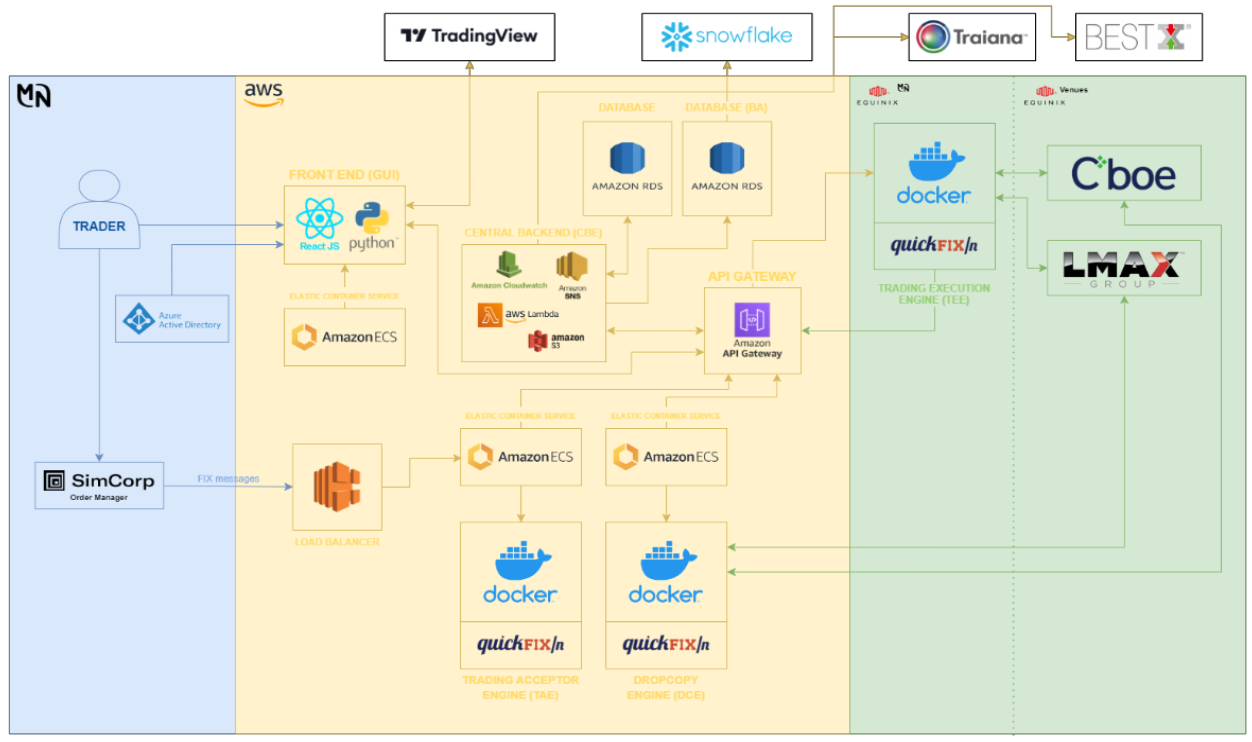
\includegraphics[width=\linewidth]{figures/Application Infrastructure.png}
%     \caption{Application Infrastructure of Algo}
%     \label{fig:application infrastructure}
% \end{figure}

The frontend, built with ReactJS and Python, provides an interface for traders and runs on AWS. Orders are processed through SimCorp Order Manager and authenticated via Azure Active Directory. The backend, hosted on AWS, handles data processing, trade execution, and market data storage using Amazon RDS and S3. It connects to the frontend and external services through an API gateway. The trading execution engine operates on Equinix, using Docker and QuickFIX/n for low-latency order processing. It connects to major venues like Cboe and LMAX Group. The system also integrates TradingView for market data, Snowflake for data storage, and Traiana and BestX for trade reconciliation and cost analysis.

\subsection{Execution Algorithm}
Putting a large order in the market all at once could result in unwanted high market impact and high costs, so instead, an order (parent order) is divided into multiple smaller child orders. These child orders are then executed according to the specific algorithm chosen by the trader. As long as child orders are not filled, they are refreshed every 50 milliseconds. 

Two execution algorithms are implemented in the Algo trading pool. They can take orders aggressively out of the order book at a certain price with a market order (resulting in spread costs) or can place limit orders in the order book, passively waiting for the order to be executed at a favorable price (resulting in opportunity costs). To maintain efficiency, child orders are refreshed every 50 milliseconds, updating their price according to market conditions while staying within the predefined limit price $L$. If the refreshed price exceeds the limit price, the order remains pending until the next update.

One algorithm is Time Weighted Average Price (TWAP) algorithm. This algorithm replicates traditional TWAP, but uses parameters to control passive, neutral and aggressive execution of child orders. It is designed to execute a trade over a fixed time period while aiming to match the time-weighted average mid-price. It splits a large order into multiple smaller child orders that are executed parallelly to minimize market impact and reduce price deviation.

TWAP algorithm requires four main inputs: the start time $t_0$, the total order volume $Q$, the execution duration $T$, and the limit price $L$. The TWAP price is defined as the time-weighted integral of the mid-price $M(t)$ over the trading period:

\begin{equation}
    p_{\text{TWAP}} = \frac{1}{T} \int_{t_0}^{t_0+T} M(t) dt.
    \label{eq: TWQP price}
\end{equation}

To approximate this price, the algorithm partitions the total volume into $n$ child orders, where $n$ is determined by the ratio of $Q$ to the minimum allowed child volume $Q_{\min}$:

\begin{equation}
    n = \left\lfloor \frac{Q}{Q_{\min}} \right\rfloor, \quad Q_n = Q - (n-1) Q_{\min}.
    \label{eq: Q_n}
\end{equation}

Each child order follows a randomized start time to reduce signaling risk. A random value $a_i$ is assigned to each child within a predefined range, and the duration of each child order is computed as:

\begin{equation}
    \delta_i = \frac{a_i T}{A}, \quad A = \sum_{i=1}^{n} a_i.
    \label{eq:sigma and A}
\end{equation}

The execution of each child order follows an adaptive approach, starting with a passive strategy and increasing aggressiveness over time. The aggressiveness is controlled by three parameters: $\alpha$, $\beta$, and $\gamma$. The order initially starts at $\alpha$ and, if unfilled, transitions to $\alpha + \beta$ after a fraction $t_{\beta}$ of its duration. If the order remains unfilled, the price fraction further increases to $\alpha + \beta + \gamma$ at time $t_{\gamma}$.

\begin{table}[h]
    \centering
    \begin{tabular}{|c|l|}
        \hline
        \textbf{Symbol} & \textbf{Description} \\ \hline
        $\alpha$ & Initial price fraction \\ \hline
        $\beta$ & Increment for the second phase \\ \hline
        $\gamma$ & Increment for the third phase \\ \hline
        $t_{\beta}$ & Time fraction before increasing aggressiveness \\ \hline
        $t_{\gamma}$ & Time fraction before final aggressiveness step \\ \hline
    \end{tabular} \label{tb:TWAP parameters}
    \caption{TWAP execution parameters}
\end{table}

In the passive mode, orders begin at $\alpha$ and transition through all phases. The neutral mode omits the passive phase and starts at $\alpha + \beta$, while the aggressive mode starts directly at the highest level of aggressiveness. This approach ensures the order is executed in a controlled manner while adapting to market conditions, reducing the risk of price deviation and improving execution efficiency.

% order placement picture in the ppt
\begin{figure}[h]
    \centering
    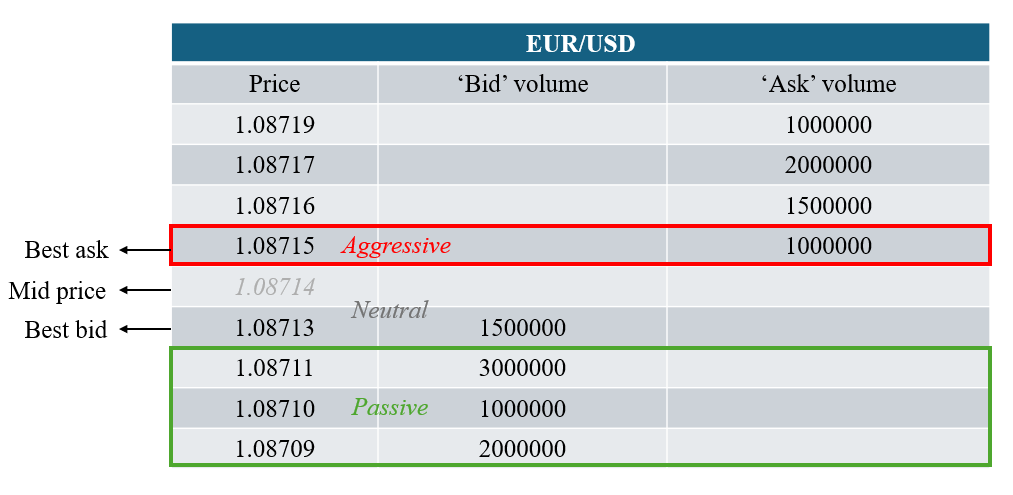
\includegraphics[width=\linewidth]{figures/order placement.png}
    \caption{Order placement of Algo}
    \label{fig:order placement}
\end{figure}

\noindent \textbf{Legend:}
\begin{itemize}
    \item Aggressive Order: Placed at the best ask.
    \item Neutral Order: Placed near the mid-price.
    \item Passive Order: Placed near the best bid.
\end{itemize}

The other one is Float algorithm. Different from TWAP, it lets the child order 'float' at a specific price level until executed. This approach reduces market impact and lowers spread costs. Since execution speed is not a priority, the algorithm is categorized as a \textit{liquidity-seeking} strategy. This algorithm allows child orders wait passively at a predefined level in the order book and adjusts its position dynamically.

The Float algorithm requires the following inputs:
\begin{itemize}
    \item A start time $t_0$.
    \item A total order volume $Q$.
    \item A price fraction $\phi$, which defines the floating position in the order book.
    \item A limit price $L$, ensuring the order does not execute at an unfavorable price.
\end{itemize}

The execution process begins by setting the remaining volume $R = Q$. The algorithm then continuously executes child orders until the total volume is filled. The volume of each child order is determined dynamically using the remaining volume:

\begin{equation}
    Q = 
    \begin{cases} 
        Q_{\text{float}}, & \text{if } R - Q_{\text{float}} \geq Q_{\text{float}}, \\
        R, & \text{otherwise}.
    \end{cases}
\end{equation}

Each child order keeps the same price fraction $\phi$ throughout its lifespan. Orders are refreshed every 50 milliseconds to ensure they remain valid under current market conditions. If a child order executes too quickly, the algorithm enforces a minimum execution duration $\delta_{\text{min}}$, delaying the next child order until sufficient time has passed.

In some cases, the market may move beyond the limit price, preventing further execution. If this happens, the order becomes stuck, meaning it will not execute unless the market returns to a favorable level. To prevent unfilled orders from persisting indefinitely, any remaining float orders are canceled at the end of each trading day.

The key differences between Float and TWAP are:
\begin{enumerate}
    \item Dynamic Timing: In TWAP, child orders have pre-defined execution times, while in Float, a new child order is only created when the previous one is filled.
    \item Remaining Volume Handling: In TWAP, unfilled portions of child orders are added to the last order. In Float, unfilled portions are returned to the remaining volume and used to calculate the next child order.
\end{enumerate}

\subsection{Parallel Venue Submission}
The MN Algo uses two trading venues: \acrshort{lmax} and \acrshort{cboe}. These venues provide real-time market updates at the millisecond level, ensuring that trading decisions are based on the most recent market conditions. 

When a trader submits an order, the execution engine determines the venue for submitting the child order. To make order submission more efficient, parallel execution is implemented to meet the business need for higher trading volume and faster execution while keeping stable spreads.

The venue submission algorithm has experienced four stages of evolution. Initially, the algorithm submitted orders to the venue with the worst best bid/ask prices. This method made sure orders are placed in the less competitive venue, so they can be filled as soon as possible. But it did not optimize execution speed or market impact. The process is illustrated in Figure~\ref{fig:venue_submission_1}, where the parent order is divided into child orders, and each child order is sent to a single venue depending on the best bis/ask prices.

\begin{figure}[h]
    \centering
    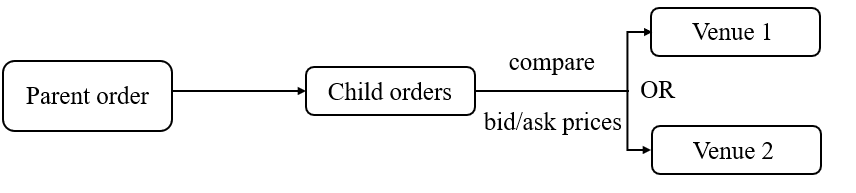
\includegraphics[width=0.8\linewidth]{figures/venue_submission_1.png}
    \caption{Initial venue submission method}
    \label{fig:venue_submission_1}
\end{figure}

A later study \citep{romy2023} found that randomly selecting a venue for each child order resulted in better performance. This randomization changed the systematic disadvantages of initial method, leading a better execution performance.

Further refinement is the use of \gls{parallel execution}, which significantly improved the performance of venue submission. Instead of submitting a single child order at a time, the algorithm places multiple child orders simultaneously across different venues. 

The first version of parallel execution split the parent order into multiple secondary parent orders, each assigned to a specific venue. Figure~\ref{fig:venue_submission_2} shows its execution process. If only one secondary order remains active, the algorithm reverts to the previous random execution method to prevent delays and ensure timely order completion. 

\begin{figure}[h]
    \centering
    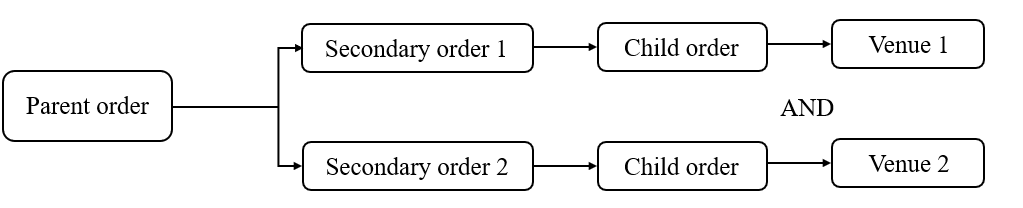
\includegraphics[width=0.8\linewidth]{figures/venue_submission_2.png}
    \caption{Parallel execution strategy version 1}
    \label{fig:venue_submission_2}
\end{figure}

Building upon this, the second version of parallel execution adjusts order execution dynamically based on venue performance. Since each venue or secondary order may have different execution speeds, the algorithm monitors execution at predefined intervals, referred to as pillars, and modifies execution settings in response to key triggers such as volume, price, and spread. The execution process is shown in Figure~\ref{fig:venue_submission_3}.
\begin{figure}[h]
    \centering
    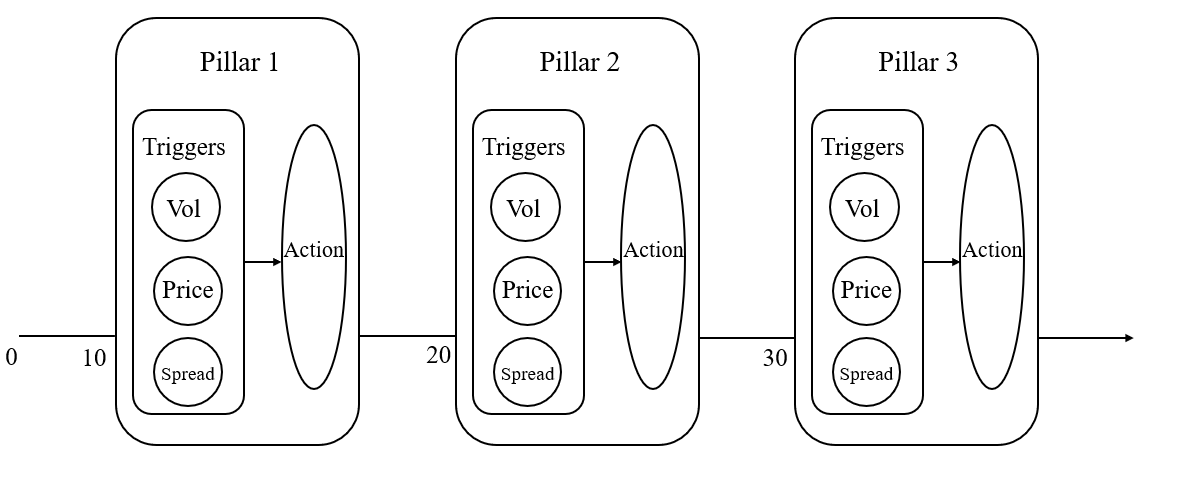
\includegraphics[width=0.8\linewidth]{figures/venue_submission_3.png}
    \caption{Parallel execution strategy version 2}
    \label{fig:venue_submission_3}
\end{figure}

% The transition from single-venue submission to randomized venue selection and ultimately to parallel execution has led to more efficient order processing, lower latency, and improved fill rates. Current parallel venue submission ensures that the trading strategy adapts to dynamic market conditions and optimizes execution quality.


\section{Back Testing}
Backtesting is a fundamental method used in quantitative trading to evaluate the performance of trading strategies based on historical market data. By simulating past trading conditions, backtesting provides evaluation of a strategy's performances before using it in live markets. A reliable backtesting environment should be both \textbf{realistic} and \textbf{dynamic}.

MN has developed a back testing environment for FX spot trading, called \textit{FX Smart Execution Backtester}. This engine is designed to assess changes in execution strategy parameters, including the optimization of child order aggressiveness and the changes of order information. 

The backtester aims to make use of complete market data:
\begin{enumerate}
    \item Historical data: Past \gls{lob} from LMAX and CBOE stored in the Snowflake.
    \item Simulated data: Synthetic \gls{lob} generated to test hidden aggressive events beyond observation.
    \item Model data: Data produced by algorithmic models to enhance market simulations.
\end{enumerate}
Currently, the backtester only uses historical \gls{lob} to execute testing of strategies. The execution engine processes order updates, places child orders at certain timestamps, and decides the rules governing order matching. The order matching rule is now based on filling possibility. The mechanism is:
\begin{itemize}
    \item Given an order information, including price, volume, trading algorithm, starting time and backtesting time range.
    \item Use best bid-ask spread to decide the filling chance of orders. As can be seen in Table~\ref{tab:filling_spread}, the narrower the spread, the higher the chance of an order being filled.
    \item Execute the order based on historical order book data.
\end{itemize} 
    \begin{table}[h]
        \centering
        \begin{tabular}{c|c|c|c|c|c|c}
            \hline
            Spread & $S \geq$ 5 & $S \geq$ 4 & $S \geq$ 3 & $S \geq$ 2 & $S \geq$ 1 & $S <$ 1 \\
            \hline
            Possibility of orders being filled & 0\% & 0.50\% & 1\% & 2\% & 5\% & 20\% \\
            \hline
        \end{tabular}
        \caption{Filling Probability and Bid-Ask Spread. Note: The spread values are in pip units, where $S=1$ corresponds to $0.0001$. Thus, $S \geq 5$ means $S \geq 0.0005$.}
        \label{tab:filling_spread}
    \end{table}



% So, whether an order would be filled or not is decided by market trend and other market participators under the simulated market order book flow. 